% !TEX TS-program = XeLaTeX
% use the following command: 
% all document files must be coded in UTF-8
\documentclass{textolivre}
% for anonymous submission
%\documentclass[anonymous]{textolivre}
% to create HTML use 
%\documentclass{textolivre-html}
% See more information on the repository: https://github.com/leolca/textolivre

% Metadata
\begin{filecontents*}[overwrite]{article.xmpdata}
    \Title{Synchronous and asynchronous distance learning of anaphora in foreign languages: an experimental study}
    \Author{Amanda Maraschin Bruscato \sep Jorge Baptista}
    \Language{en-US}
    \Keywords{anaphora \sep distance learning modalities \sep foreign languages learning}
    \Journaltitle{Texto Livre}
    \Journalnumber{1983-3652}
    \Volume{14}
    \Issue{1}
    \Firstpage{1}
    \Lastpage{16}
    \Doi{10.35699/1983-3652.2021.29177}

    \setRGBcolorprofile{sRGB_IEC61966-2-1_black_scaled.icc}
            {sRGB_IEC61966-2-1_black_scaled}
            {sRGB IEC61966 v2.1 with black scaling}
            {http://www.color.org}
\end{filecontents*}

% used in this example to provide source code environment
%\crefname{lstlisting}{lista}{listas}
%\Crefname{lstlisting}{Lista}{Listas}
%\usepackage{listings}
%\renewcommand\lstlistingname{Lista}
%\lstset{language=bash,
        breaklines=true,
        basicstyle=\linespread{1}\small\ttfamily,
        numbers=none,xleftmargin=0.5cm,
        frame=none,
        framexleftmargin=0.5em,
        framexrightmargin=0.5em,
        showstringspaces=false,
        upquote=true,
        commentstyle=\color{gray},
        literate=%
           {á}{{\'a}}1 {é}{{\'e}}1 {í}{{\'i}}1 {ó}{{\'o}}1 {ú}{{\'u}}1 
           {à}{{\`a}}1 {è}{{\`e}}1 {ì}{{\`i}}1 {ò}{{\`o}}1 {ù}{{\`u}}1
           {ã}{{\~a}}1 {ẽ}{{\~e}}1 {ĩ}{{\~i}}1 {õ}{{\~o}}1 {ũ}{{\~u}}1
           {â}{{\^a}}1 {ê}{{\^e}}1 {î}{{\^i}}1 {ô}{{\^o}}1 {û}{{\^u}}1
           {ä}{{\"a}}1 {ë}{{\"e}}1 {ï}{{\"i}}1 {ö}{{\"o}}1 {ü}{{\"u}}1
           {Á}{{\'A}}1 {É}{{\'E}}1 {Í}{{\'I}}1 {Ó}{{\'O}}1 {Ú}{{\'U}}1
           {À}{{\`A}}1 {È}{{\`E}}1 {Ì}{{\`I}}1 {Ò}{{\`O}}1 {Ù}{{\`U}}1
           {Ã}{{\~A}}1 {Ẽ}{{\~E}}1 {Ũ}{{\~u}}1 {Õ}{{\~O}}1 {Ũ}{{\~U}}1
           {Â}{{\^A}}1 {Ê}{{\^E}}1 {Î}{{\^I}}1 {Ô}{{\^O}}1 {Û}{{\^U}}1
           {Ä}{{\"A}}1 {Ë}{{\"E}}1 {Ï}{{\"I}}1 {Ö}{{\"O}}1 {Ü}{{\"U}}1
           {ç}{{\c{c}}}1 {Ç}{{\c{C}}}1
}


\journalname{Texto Livre: Linguagem e Tecnologia}
\thevolume{14}
\thenumber{1}
\theyear{2021}
\receiveddate{\DTMdisplaydate{2020}{10}{22}{-1}} % YYYY MM DD
\accepteddate{\DTMdisplaydate{2020}{9}{3}{-1}}
\publisheddate{\today}
% Corresponding author
\corrauthor{Amanda M. Bruscato }
% DOI
\articledoi{10.35699/1983-3652.2021.29177}
% Abbreviated author list for the running footer
\runningauthor{Bruscato and Baptista}
\editorname{Leonardo Araújo}

\title{Synchronous and asynchronous distance learning of anaphora in foreign languages: an experimental study}
\othertitle{Ensino síncrono e assíncrono a distância de anáfora em línguas estrangeiras: um estudo experimental}
% if there is a third language title, add here:
%\othertitle{Artikelvorlage zur Einreichung beim Texto Livre Journal}

\author[1]{Amanda Maraschin Bruscato \orcid{0000-0003-0660-9098} \thanks{Email: \url{amandabruscato@gmail.com}}}
\author[1,2]{Jorge Baptista \orcid{0000-0003-4603-4364} \thanks{Email: \url{jbaptis@ualg.pt}}}

\affil[1]{Universidade do Algarve, Portugal.}
\affil[2]{Instituto de Engenharia de Sistemas e Computadores, Investigação e Desenvolvimento em Lisboa, Portugal.}

\addbibresource{article.bib}
% use biber instead of bibtex
% $ biber tl-article-template

% set language of the article
\setdefaultlanguage{english}
\setotherlanguage{portuguese}

% for spanish, use:
%\setdefaultlanguage{spanish}
%\gappto\captionsspanish{\renewcommand{\tablename}{Tabla}} % use 'Tabla' instead of 'Cuadro'

% for languages that use special fonts, you must provide the typeface that will be used
% \setotherlanguage{arabic}
% \newfontfamily\arabicfont[Script=Arabic]{Amiri}
% \newfontfamily\arabicfontsf[Script=Arabic]{Amiri}
% \newfontfamily\arabicfonttt[Script=Arabic]{Amiri}
%
% in the article, to add arabic text use: \textlang{arabic}{ ... }

% to use emoticons in your manuscript
% https://stackoverflow.com/questions/190145/how-to-insert-emoticons-in-latex/57076064
% using font Symbola, which has full support
% the font may be downloaded at:
% https://dn-works.com/ufas/
% add to preamble:
% \newfontfamily\Symbola{Symbola}
% in the text use:
% {\Symbola 😥}


%%%% reference item description using its label instead of numbers
%%% BEGIN
%\makeatletter
%\let\orgdescriptionlabel\descriptionlabel
%\renewcommand*{\descriptionlabel}[1]{%
%  \let\orglabel\label
%  \let\label\@gobble
%  \phantomsection
%  \edef\@currentlabel{#1\unskip}%
%  \let\label\orglabel
%  \orgdescriptionlabel{#1}%
%}
%\makeatother
%%% END


%%%% possessive textcite
%%% BEGIN
%\DeclareCiteCommand*{\citeauthor}%
%  {\boolfalse{citetracker}%
%   \boolfalse{pagetracker}%
%   \usebibmacro{prenote}}%
%  {\ifciteindex%
%     {\indexnames{labelname}}%
%     {}%
%   \printtext[bibhyperref]{\printnames[firstword]{labelname}}}%
%  {\multicitedelim}%
%  {\usebibmacro{postnote}}%

%\newcommand\posscite[1]{\expandafter\MakeLowercase\expandafter{\citeauthor*{#1}}'s \citeyear{#1}}
%\newcommand\posscite[1]{\lowercase\expandafter{\citeauthor*{#1}}'s \citeyear{#1}}
%\newcommand\posscite[1]{\citeauthor*{#1}'s \citeyear{#1}}
%\DeclareNameWrapperFormat{textlabelname:poss}{#1's}
%
%\DeclareFieldFormat{shorthand:poss}{%
%  \ifnameundef{labelname}{#1's}{#1}}
%
%\DeclareFieldFormat{citetitle:poss}{\mkbibemph{#1}'s}
%
%\DeclareFieldFormat{label:poss}{#1's}
%
%\newrobustcmd*{\posscitealias}{%
%  \AtNextCite{%
%    \DeclareNameWrapperAlias{labelname}{textlabelname:poss}%
%    \DeclareFieldAlias{shorthand}{shorthand:poss}%
%    \DeclareFieldAlias{citetitle}{citetitle:poss}%
%    \DeclareFieldAlias{label}{label:poss}}}
%
%\newrobustcmd*{\posscite}{%
%  \posscitealias%
%  \textcite}
%
%\newrobustcmd*{\Posscite}{\bibsentence\posscite}
%
%\newrobustcmd*{\posscites}{%
%  \posscitealias%
%  \textcites}
%%% END



\usepackage{multirow}

\begin{document}
\maketitle

\begin{polyabstract}
\begin{abstract}
This paper analyses the influence of the distance learning modality
(synchronous/asynchronous) in the learning of anaphora in English and Spanish
as foreign languages, based on the results of a course offered to 45 Modern
Language students at a Brazilian university in the first semester of 2020.
Factors as the level of proficiency, type of task, and degree of motivation
were also considered in this experimental study. Two experimental groups and
one control group were compared in four written tests. English learners
demonstrated a higher prior knowledge of anaphora than Spanish learners and
showed the best test results. A positive and moderate correlation was found
between the knowledge of anaphora, level of proficiency, and degree of
motivation to study the language. Although the experimental groups made
progress in the reading tests, the same did not happen in the writing tests.
Finally, the difference was not significant between the two experimental
groups.

\keywords{anaphora \sep distance learning modalities \sep foreign languages learning}
\end{abstract}

\begin{portuguese}
\begin{abstract}
Este artigo pretende analisar a influência da modalidade de ensino a distância
(síncrona e assíncrona) na aprendizagem da anáfora em inglês e espanhol como
línguas estrangeiras, com base nos resultados de um curso oferecido a 45
estudantes de Letras de uma universidade brasileira no primeiro semestre de
2020. Neste estudo experimental, também foram considerados fatores como o nível
de proficiência, grau de motivação e tipo de tarefa. Dois grupos experimentais
e um grupo de controle foram comparados, ao longo de quatro testes. Os
estudantes de inglês demonstraram maior conhecimento prévio de anáfora do que
os de espanhol e apresentaram melhores resultados nos testes. Identificou-se
uma correlação positiva e moderada entre o conhecimento de anáfora, o nível de
proficiência e o grau de motivação para estudar a língua. Apesar de os grupos
experimentais progredirem nos testes de compreensão, o mesmo não ocorreu nos
testes de produção escrita. Por fim, não houve diferença significativa entre os
dois grupos experimentais.

\keywords{anáfora \sep modalidades de ensino a distância \sep aprendizagem de línguas estrangeiras}
\end{abstract}
\end{portuguese}

% if there is another abstract, insert it here using the same scheme
\end{polyabstract}


\section{Introduction}\label{sec-intro}
In 2020, many educational institutions around the world had to adapt their
classes to the distance learning environment because of the COVID-19
(Coronavirus Disease 2019) pandemic. In a recent study, \textcite{bruscato_teaching_2020} 
have found that students and professors at different Brazilian and
Portuguese universities have a negative perception about distance learning.
However, since it is the safest option during the pandemic, it is necessary to
investigate if the synchronous or asynchronous modalities have different
effects on learning outcomes.

For this article, we have decided to investigate how the learning of anaphora
in English and Spanish as foreign languages is affected by synchronous and
asynchronous learning. We also aim to answer how it is affected by students’
motivation and proficiency in the languages. It is possible that Portuguese
native speakers have better outcomes when learning Spanish, since these
languages are more similar than Portuguese and English, and that students with
higher motivation and proficiency levels may have the highest learning
outcomes. We also believe that students from the asynchronous group may have
better outcomes, since they have more chances to practice their reading and
writing on forums than students from the synchronous group, who will be
listening and speaking on videoconferences.

Thus, this study addresses the following research questions (Q): Are there
differences in the learning of anaphora depending on (Q1) the distance learning
modality; (Q2) the foreign language studied; (Q3) the assessment of reading or
writing; (Q4) the level of proficiency in the foreign language; and (Q5) the
participants’ degree of motivation?

To answer these questions, a short course was taught in the first semester of
2020 to 45 undergraduate students with a major in English or Spanish at the
Federal University of Rio Grande do Sul. Participants with
intermediate/advanced level in the languages were randomly assigned into two
experimental groups and one control group, and their learning outcomes were
statistically compared based on four written tests. An initial questionnaire
was applied, 2 lessons were offered, and 4 written tests were performed.

Anaphora is an important cohesive mechanism, and its knowledge is indispensable
for communication in the language. Instead of overusing nominal repetition, as
in \ref{itm-1a}, speakers can use pronouns \ref{itm-1b}, or ellipsis \ref{itm-1c}, to refer to the
antecedent in the text.

%
% LIST
%
%\begin{description}[topsep=1ex,partopsep=1ex]
%  \item[(1a)\label{itm-1a}] Anna\textsubscript{i} wakes up every morning and Anna\textsubscript{i} goes to work. 
%  \item[(1b)\label{itm-1b}] Anna\textsubscript{i} wakes up every morning and she\textsubscript{i} goes to work.
%  \item[(1c)\label{itm-1c}] Anna\textsubscript{i} wakes up every morning and Ø\textsubscript{i} goes to work.
%\end{description}
\begin{enumerate}[wide,label=(\arabic*),topsep=1ex,partopsep=1ex,leftmargin=0.15cm,noitemsep]
\setlength{\itemindent}{0em}
\item[]{} \addtocounter{enumi}{1} %\setcounter{enumi}{2}
\begin{enumerate}[wide,label=(\arabic{enumi}\alph*),topsep=1ex,partopsep=1ex,noitemsep]
\setlength{\itemindent}{0em}
\item \label{itm-1a} Anna\textsubscript{i} wakes up every morning and Anna\textsubscript{i} goes to work.
\item \label{itm-1b} Anna\textsubscript{i} wakes up every morning and she\textsubscript{i} goes to work.
\item \label{itm-1c} Anna\textsubscript{i} wakes up every morning and Ø\textsubscript{i} goes to work.
\end{enumerate}
\end{enumerate}


English and Spanish are the most widely spoken European languages in the world
\cite{eberhard_ethnologue:_2020} and differ from each other in terms of
anaphora resolution strategies, for example by the use or not of grammatical
gender and by the Null Subject Parameter \cite{chomsky_lectures_1981,rizzi_issues_1982}. Besides
teaching the main anaphora processes in these two languages, the course was
designed to collect data on the students' learning progress in relation to this
linguistic mechanism. The legally required authorizations were obtained from
the institution; students were informed accordingly, and all agreed to
participate in the research on a voluntary basis.

In the next two sections, a brief literature review on anaphora and on distance
learning will be presented. Then, the research method will be described and,
finally, the results will be discussed. The article ends with the establishment
of conclusions and indications for future work.

\section{Anaphora}\label{sec-anaphora}
In the \emph{Common European Framework of Reference for Languages} \cite[p. 140]{council_of_europe_common_2009},
types of anaphora are considered forms of textual cohesion that
should be taught to all language learners, especially from level B1. The
document is used alongside specific frameworks in the development of national
curricula and proficiency tests. These tests assess proficiency in the use of
anaphora by integrating it into the criteria used to measure the learner's
knowledge of textual cohesion.

\emph{Cohesion} is defined by \textcite[p. 4]{halliday_cohesion_1976} as the relations
of meaning in the text, which can be established by using a linguistic element
(\emph{anaphor}) dependent semantically on the element to which it refers
(\emph{antecedent}). Grammatical reference can be \emph{exophoric} if it concerns something
outside the text, as seen in \ref{itm-2}, below, where the pronoun this refers to
something extralinguistic; or it can be \emph{endophoric} if the antecedent is in the
text, as seen in \ref{itm-3a} and \ref{itm-3b}. The endophoric reference may be \emph{anaphoric} if
the anaphor takes up a previously mentioned antecedent, as in the case of (3a),
in which the pronoun \emph{it} refers to \emph{a pen}; or \emph{cataphoric} if it anticipates
something that will soon be mentioned, case of \ref{itm-3b}, in which the pronoun \emph{this}
refers to \emph{be gentle}.

%
% LIST
%
%\begin{description}[topsep=1ex,partopsep=1ex]
%  \item[(2)\label{itm-2}] This does not belong to me. 
%  \item[(3a)\label{itm-3a}] I found a pen\textsubscript{i}, but it\textsubscript{i} does not belong to me. 
%  \item[(3b)\label{itm-3b}] I just say this\textsubscript{i}: be gentle\textsubscript{i}.
%\end{description}

\begin{enumerate}[wide,label=(\arabic*),topsep=1ex,partopsep=1ex,noitemsep,leftmargin=0.15cm,resume]
\setlength{\itemindent}{0em}
\item \label{itm-2} This does not belong to me.
\item[]{} \addtocounter{enumi}{1} 
\begin{enumerate}[wide,label=(\arabic{enumi}\alph*),topsep=1ex,partopsep=1ex,noitemsep]
\setlength{\itemindent}{0em}
\item \label{itm-3a} I found a pen\textsubscript{i}, but it\textsubscript{i} does not belong to me.
\item \label{itm-3b} I just say this\textsubscript{i}: be gentle\textsubscript{i}.
\end{enumerate}
\end{enumerate}

\textcite{halliday_cohesion_1976} differentiate grammatical cohesion from
lexical cohesion (where there is nominal repetition) and separate
\emph{reference} from \emph{substitution}. According to the authors,
reference would establish semantic relations, while substitution would
establish grammatical relations. They also present the \emph{ellipsis},
seen in \ref{itm-4}, apart from substitution, exemplified in \ref{itm-5}, although they
agree that ellipsis may be a type of substitution. In \ref{itm-4}, there is the
elision of \emph{coffee} in the second clause, and in \ref{itm-5}, the
\emph{same} refers to \emph{order} \emph{a coffee.} After the examples,
the authors' types of cohesion are presented in \Cref{fig01}.


%
% LIST
%
%\begin{description}[topsep=1ex,partopsep=1ex]
%  \item[(4)\label{itm-4}] I want to order a coffee\textsubscript{i}, I imagine she wants to order another Ø\textsubscript{i}. 
%  \item[(5)\label{itm-5}] I want to order a coffee\textsubscript{i}, I imagine she wants the same\textsubscript{i}. 
%\end{description}
\begin{enumerate}[wide,label=(\arabic*),topsep=1ex,partopsep=1ex,noitemsep,leftmargin=0.15cm,resume]
\setlength{\itemindent}{0em}
\item[]{} \addtocounter{enumi}{1}
\begin{enumerate}[wide,label=(\arabic{enumi}\alph*),topsep=1ex,partopsep=1ex,noitemsep]
\setlength{\itemindent}{0em}
\item \label{itm-4} I want to order a coffee\textsubscript{i}, I imagine she wants to order another Ø\textsubscript{i}.
\item \label{itm-5} I want to order a coffee\textsubscript{i}, I imagine she wants the same\textsubscript{i}. 
\end{enumerate}
\end{enumerate}




%
% FIGURE 1
% 
\begin{figure}[htbp]
 \centering
 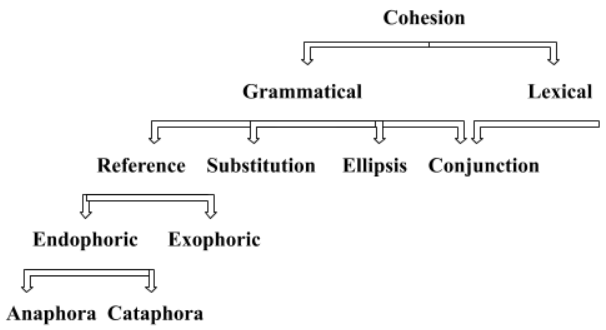
\includegraphics[width=0.75\textwidth]{fig01.png}
 \caption{Cohesion.}
 \label{fig01}
 \source{\textcite{halliday_cohesion_1976}.}
\end{figure}



Based on \textcite{halliday_cohesion_1976}, the Brazilian authors \textcite{favero_criterios_1985}
proposed a new classification of cohesion, dividing it into
referential, sequential, and lexical. After the publication of their
study, however, the authors reviewed their positions and reclassified
cohesion, each in their own way. \textcite{favero_coesao_2010} divided it into
referential, sequential, and recurrent; while \textcite{koch_coesao_2010} divided it
only into referential and sequential.

According to \textcite[p. 18-25]{favero_coesao_2010}, \emph{referential cohesion} - the
focus of this paper - occurs when the interpretation of a linguistic
element depends on the interpretation of the element to which it refers,
either by substitution or reiteration. While referential cohesion by
\emph{reiteration} uses the repetition of expressions in the text, seen
in \ref{itm-5a}, referential cohesion by \emph{substitution} is achieved by
ellipsis (zero anaphora), exemplified in \ref{itm-5b}, or by a \emph{pro-form,
i.e.,} a grammatical element that carries the meaning of the element it
replaces \cite[p. 19]{favero_coesao_2010}, as seen in \ref{itm-5c}. After the examples, the
author's types of cohesion are presented in \Cref{fig02}.

%
% LIST
%
%\begin{description}[topsep=1ex,partopsep=1ex]
%  \item[(5a)\label{itm-5a}] Mary\textsubscript{i} went to the theater and Mary\textsubscript{i} did not like the play. 
%  \item[(5b)\label{itm-5b}] Mary\textsubscript{i} went to the theater and Ø\textsubscript{i} did not like the play.
%  \item[(5c)\label{itm-5c}] Mary\textsubscript{i} went to the theater and she\textsubscript{i} did not like the play.
%\end{description}
\begin{enumerate}[wide,label=(\arabic*),topsep=1ex,partopsep=1ex,noitemsep,leftmargin=0.15cm,resume]
\setlength{\itemindent}{0em}
\item[]{} \addtocounter{enumi}{1}
\begin{enumerate}[wide,label=(\arabic{enumi}\alph*),topsep=1ex,partopsep=1ex,noitemsep]
\setlength{\itemindent}{0em}
\item \label{itm-5a} Mary\textsubscript{i} went to the theater and Mary\textsubscript{i} did not like the play.
\item \label{itm-5b} Mary\textsubscript{i} went to the theater and Ø\textsubscript{i} did not like the play.
\item \label{itm-5c} Mary\textsubscript{i} went to the theater and she\textsubscript{i} did not like the play.
\end{enumerate}
\end{enumerate}



% 
% FIGURE 2
%
\begin{figure}[htbp]
 \centering
 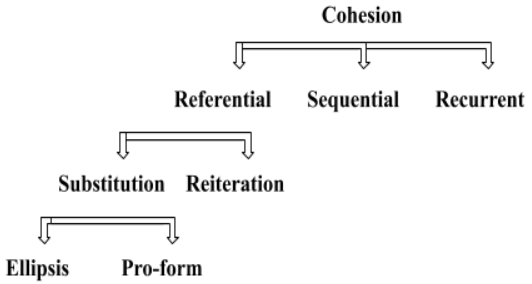
\includegraphics[width=0.75\textwidth]{fig02.png}
 \caption{Cohesion.}
 \label{fig02}
 \source{\textcite{favero_coesao_2010}.}
\end{figure}




In this article, the learning of referential cohesion, referred here as
\emph{anaphora}, will be investigated. The research focuses on the
learning of anaphora in English and Spanish as foreign languages by
Brazilian Portuguese native speakers. It is possible that, due to the
similarity of Portuguese and Spanish in relation to grammatical gender
and the Null Subject Parameter \cite{chomsky_lectures_1981,rizzi_issues_1982} -- which
allows the omission of the subject in various contexts -, Brazilian
students may find it easier to solve anaphora in Spanish than in
English.

The process of interpreting the anaphor is also called \emph{anaphora
resolution} \cite{hirstanaphora1981,mcdonald_time_1995,mitkov_oxford_2005} 
and it can be study from different linguistic perspectives, such as
syntactic, semantic, and pragmatic \cite{ariel_interpreting_1994,arnold_effect_2001,grosz_centering:_1995,rahman_coreference_2011}.
Even so, it can be said 
that scholars in general tend to agree with the definition of anaphora
as the relation between linguistic elements, where the interpretation of
the anaphor depends on the interpretation of its antecedent \cite[p. 1]{huanganaphora2000}.

The perspectives described above (Halliday and Hassan, Fávero and Koch)
are semantic-discursive, considering not only the intraphrasic context
but also the transfrastic, which covers more than one sentence. In our
study, we adopt the multi-strategic approach proposed by \textcite{carbonell_anaphora_1988}.
The authors explain that anaphora resolution is not an
exclusively morphological, syntactic, semantic, or pragmatic process,
but that it integrates these various dimensions. They then define
preferences and restrictions of these four orders as criteria for the
resolution of anaphora. For example, in \ref{itm-6a}, due to semantic
restrictions, it is known that the pronoun \emph{it} refers to \emph{the
pie}; but in \ref{itm-6b}, it is known that \emph{it} refers to \emph{the
table}. In addition to the semantic restriction, there are gender and
number restrictions in this case, as \emph{it} could not refer to a
person nor to more than one antecedent.

%
% LIST
%
%\begin{description}[topsep=1ex,partopsep=1ex]
%  \item[(6a)\label{itm-6a}] John took the pie\textsubscript{i} off the table and ate it\textsubscript{i}.  
%  \item[(6b)\label{itm-6b}] John took the pie off the table\textsubscript{i} and cleaned it\textsubscript{i}. 
%\end{description}
\begin{enumerate}[wide,label=(\arabic*),topsep=1ex,partopsep=1ex,noitemsep,leftmargin=0.15cm,resume]
\setlength{\itemindent}{0em}
\item[]{} \addtocounter{enumi}{1} 
\begin{enumerate}[wide,label=(\arabic{enumi}\alph*),topsep=1ex,partopsep=1ex,noitemsep]
\setlength{\itemindent}{0em}
\item \label{itm-6a} John took the pie\textsubscript{i} off the table and ate it\textsubscript{i}.
\item \label{itm-6b} John took the pie off the table\textsubscript{i} and cleaned it\textsubscript{i}.
\end{enumerate}
\end{enumerate}


Several studies have analysed anaphora resolution in the context of
foreign languages learning, many through the analysis of learner
corpora. A learner corpus is a collection of linguistic data
produced by learners of a foreign language \cite[p. 65]{mcenery_corpus_2006}.
According to \textcite[p. 288]{mitchell_second_2013}, the
use of electronic corpora and computer tools allows for a better
and more systematic analysis of grammatical learning processes in a
second language learning context.

\textcite{lozano_2016} investigated the use of anaphora in the \emph{Corpus
Escrito del Español L2} and showed that learners consider it more
important that the content communicated is clear and unambiguous than
concise. They prefer, therefore, to make explicit the subject to
eliminate any possible ambiguity than to leave some doubt as to its
antecedent.

\textcite{pretorius_english_2005} investigated the relationship between university
students' academic performance, proficiency in English as a second
language, and knowledge of anaphora. The author discovered that the
participants with less knowledge of anaphora did not have a good
academic performance and suggested that, without the understanding of
the cohesive mechanism, it was because they could not effectively
understand the readings required in the course. The author also found
that, in higher levels of proficiency in the second language, the
differences between students' knowledge of anaphora were smaller. This
research demonstrated the relevance of anaphora for reading in the
foreign language and academic performance.

\textcite[p. 608-9]{ellis_study_2008} presents a compilation of studies that have
investigated foreign language learners' knowledge of anaphora. However,
they do not analyse the impact of teaching or the learning modality.
Research on this topic will therefore be discussed in the next section.


\section{Distance learning}\label{sec-dist-learn}
Distance learning, currently possible using the New Information and
Communication Technologies, can be carried out through synchronous or
asynchronous lessons. In the first case, individuals must be connected
at the same time to participate in video conferences and chats. In the
second case, they can watch video lessons, answer exercises, and
participate in discussion forums at different times. The two modalities
have opposite advantages and disadvantages: while the synchronous class
allows live contact between participants and further development of oral
production but restricts the possibility of access to a certain day and
time; the asynchronous class makes access more flexible and provides
further development of written production but does not offer live
contact.

The distance learning modalities have been studied by several authors,
such as \textcite{chou_comparative_2002,skylar_comparison_2009}. \textcite{chou_comparative_2002} analysed the
interaction between students in synchronous and asynchronous classes.
The author concluded that smaller groups interact more and that students
spend more time interacting in asynchronous discussions than in
synchronous ones. In \posscite{skylar_comparison_2009} survey, 44 students participated in
both the synchronous and asynchronous course. Both modalities were
effective for learning, though most students preferred synchronous
lessons because of the greater interactivity with the teacher and their
peers.

Specifically on foreign languages, \textcite{chen_adoption_2007} compared
synchronous and asynchronous learning using \posscite{krashen1982} theory of
second language acquisition. According to the authors, synchronous
learning allows for more communication and natural language acquisition,
while asynchronous learning allows for greater access to extra materials
and automatic exercises, as well as it offers students more time to
study and to correct their own productions. Similarly, \posscite{sotillo_discourse_2000}
concluded from her study with 25 English learners that synchronous
discussions allow for more spontaneous interaction, while asynchronous
discussions allow students to review their writing.

Although many studies have analysed foreign language learners' knowledge
of anaphora and others (which will continue to be discussed below) have
analysed the impact of the learning modality on language learning, few
studies have linked these two topics, which is the aim of this paper.

Some reviews on the effectiveness of Computer Assisted Language Learning
(CALL) in recent decades have been undertaken by \textcite{stockwell_review_2007}  %Stockwell (2007) 
and \textcite{liu_look_2002}. Other literature reviews have
analysed the impact of CALL specifically on the teaching of reading
\cite{kim_use_2002} or writing \cite{yang_review_2012} in English. Although
CALL can be used in synchronous and asynchronous learning, in this
paper, we use the term to refer to the asynchronous distance learning
modality.

\textcite{macaro_systematic_2012} compiled the research on the impact
of CALL on foreign language school education from 1990 to 2010. A total
of 117 studies were found, of which 90 dealt with English teaching. The
authors selected, for a more detailed analysis, the 47 publications of
this century on English teaching in schools. They criticized the quality
of research due to methodological flaws. As an example, they mentioned
studies that affirmed progress in student learning but did not conduct
initial tests with students, as well as others that did not compare the
data of an experimental group with that of a control group.

Despite the existence of several investigations on the impact of the
learning modality on foreign language learning, only two publications
were found which dealt specifically with the impact of the learning
modality on the learning of anaphora. According to \textcite[p. 72]{li_engaging_2014}, in
previous research, CALL has proved to have a positive impact on reading
in foreign languages, but little has been investigated about its
effectiveness in learning discursive mechanisms such as anaphora.

\textcite{liu_acquisition_2010} investigated whether the type of \emph{feedback} used in CALL
would have any impact on the learning of pronominal anaphora in English
as a second language. 28 Chinese students, aged between 19 and 40 and
with intermediate proficiency in English, participated in this research.
The participants took an initial test, computer exercises on anaphora
for half an hour, and finally a final test. One group received the
explanatory \emph{feedback} (besides right/error, the explanation of the
error) and the other group received only the message of "right" or
"wrong". There were no differences between the results of the two
groups. However, the two tests applied were the same, which may have
compromised the results.

Although \textcite{liu_acquisition_2010} concluded from his research that the explanatory
\emph{feedback} did not lead to differences in student learning, other
studies have shown the opposite \cite{lyster_corrective_1997,heift_corrective_2004,mackey_pushing_2006}. 
Though there is no consensus on the impact of the
types of \emph{feedback} on learning, it was decided that the
\emph{feedback} offered in the course exercises for all learning
modalities would be of an explanatory nature. The explanatory
\emph{feedback} is defined as \emph{metalinguistic} by \textcite[p. 47]{lyster_corrective_1997}
and seems to be the most appropriate for this research as
the participants are undergraduate students with a major in modern
languages who need to know and use grammatical terms in their
profession.

While \textcite{liu_acquisition_2010} studied the impact of computer \emph{feedback} on the
learning of anaphora in English, \textcite{li_engaging_2014} compared the learning of zero
anaphora in Chinese as a foreign language depending on the learning
modality. Her research, however, considered only the understanding of
anaphora in Chinese, not its production, and compared asynchronous
learning with in-person learning. During two weeks, 45 university
students from the United States of America who had their regular
in-person Chinese classes were divided into three groups: one that
received in-person instruction on anaphora; one that received
instruction through CALL; and one that did not receive any instruction
on the topic. The participants answered a questionnaire, a pretest, an
immediate posttest, and a delayed posttest after one month. The CALL
group obtained the best results, followed by the in-person group, and
finally by the control group. The author suggested that the CALL
students, probably due to the learning modality, demonstrated greater
autonomy, dedication, and interest in the learning.

The present article aims to investigate the impact of synchronous and
asynchronous distance learning modalities in the learning of anaphora in
English and Spanish reading and writing. The following section will
explain the research method adopted.


\section{Method}\label{sec-method}
As explained in the introduction, this paper aims to answer whether
there are differences in the learning of anaphora depending on: the
distance learning modality (Q1); the foreign language studied (Q2); the
assessment of reading or writing (Q3); the level of proficiency in the
foreign language (Q4); and the participants' degree of motivation (Q5).

This longitudinal study used the experimental method and statistically
analyses quantitative data collected from learners. Before it was
carried out, the project received approval from the university ethical
board. A total of 45 undergraduate students at the Federal University of
Rio Grande do Sul with a major in English or Spanish and with an
intermediate/advanced knowledge of the language volunteered to
participate in the research. The distribution of the sample by group is
presented in the \Cref{tbl01}. The majority was female (73\%) and the
median age was 20 years old (age varied between 18 and 41 years old).
Most of them studied English (67\%) and were in the third semester
(62\%) of their course. The number of participants does not allow the
results to be generalised, but it offers data for preliminary analysis.

\begin{table}[htpb]
\caption{Distribution of the sample by group.}
\label{tbl01}
\centering
\begin{tabular}{lllll}
\toprule
Language & \multicolumn{2}{l}{Spanish} & \multicolumn{2}{l}{English} \\
\midrule 
Group & III & V & III & V\\
Synchronous & 2 & 3 & 7 & 3\\
Asynchronous & 3 & 2 & 7 & 3\\
Control & 2 & 3 & 7 & 3\\
\bottomrule
\end{tabular}
\source{Own elaboration.}
\end{table}


For each language, students from the third and fifth semesters were
randomly distributed between two experimental groups and one control
group. The experimental groups participated in two lessons on anaphora
in their target language (independent variable), and test results from
the three groups were compared (dependent variable). The university
e-learning platform (\emph{Moodle}) was used for the lessons. Each
synchronous lesson used videoconference for 90 minutes; for asynchronous
lessons, short videos, texts, discussion forums, and automatic exercises
were used.

After signing the Informed Consent Form, all participants answered the
\emph{Motivated Strategies for Learning Questionnaire}, developed by
\textcite{pintrich_reliability_1993} and translated, reduced,
and validated in Portuguese by \textcite{mckeachie_2008}; a
proficiency test with 20 reading questions, taken from Cambridge
University or Cervantes Institute, equally distributed between levels A2
and C1; and 4 written tests which measured students' knowledge of
anaphora in the foreign language. There was a pretest before the first
lesson, a first posttest after the first lesson, a second posttest after
the second lesson, and a third posttest one month after the end of the
course.

The MSLQ is measured by a 7-point Likert scale, from 1 (completely
false) to 7 (completely true), and has, in the Portuguese version, 28
items divided in the \emph{Motivation} and \emph{Learning Strategies}
sections. The first includes the \emph{Value}, \emph{Expectancy}, and
\emph{Affective} Components; the second includes the \emph{Cognitive and
Metacognitive Strategies}, and \emph{Resource Management Strategies}.
Each component/strategy includes certain constructs, in which the items
are framed. Except for the \emph{Test Anxiety} construct, a positive
score represents a positive result.

Each lesson in this study (intervention
with the experimental groups) included the following moments: activation
of prior knowledge on the topic; lecture on anaphora for half an hour;
reading and analysis of material; group discussion; reading and writing
exercises; and feedback. Some practical differences between synchronous
and asynchronous modalities were: the lecture, which was either live or
recorded; the discussions, which took place orally live or in written
forums; and the feedback, which was done after all the students in the
class had finished each activity or automatically on the computer after
each exercise. While synchronous learning allows for a greater contact
between peers and with the teacher, asynchronous learning allows for
automatic feedback and access to a greater amount of information, in
addition, of course, to flexibility of time.

In the first lesson, students introduced themselves; learned about
cohesion; the types of anaphora; and the subject, object, and possessive
pronouns in the language of study; worked with corpus; completed
sentences with the correct pronouns; and did an exercise similar to the
test. In the second lesson, they were challenged to solve the ambiguity
of some sentences; learned about ambiguity resolution, demonstrative,
and relative pronouns; corrected and completed some sentences with
pronouns; analysed the coreferences in a fable, comparing their manual
analysis with an automatic one; and, again, they did an exercise like
the test. The designing of the course is further discussed in \textcite{bruscato_designing_2021}.

The tests had two parts: first, students had to read the beginning of a
narrative and correct the mistakes they found (there were 10 different
errors of anaphora -- wrong anaphors). Then, they should write an end to
the story (100-150 words). Since the four tests should be comparable,
the narratives were written by the researchers and validated by English
and Spanish native speakers. The 10 types of errors (distributed
differently in the texts) were: (e1) an unnecessary subject pronoun;
(e2) a missing indirect object pronoun in Spanish or a subject pronoun
in English; (e3) an unnecessary nominal repetition; (e4) a pronoun
instead of a possessive determinant; (e5) a wrong demonstrative; (e6) a
wrong relative pronoun; (e7) a reflexive pronoun missing in Spanish or
used unnecessarily in English; (e8) a masculine determinant instead of a
neuter pronoun in Spanish or an object pronoun instead of a possessive
determinant in English; (e9) a personal pronoun used to retake a
non-human antecedent; (e10) and a determinant before a relative pronoun
in Spanish or a subject pronoun instead of an object pronoun in
English.

The different types of errors in the texts are highlighted in bold
below.

\vspace{1ex}
\begin{samepage}
Text in English:

\nopagebreak
\emph{John and Mary were twins and \textbf{they were}} (e1) \emph{only
twelve years old whe\textbf{n}} (e2) \emph{\textbf{b}ecame orphans.
Before \textbf{these}} (e5) \emph{misfortune, \textbf{John and Mary}}
(e3) \emph{lived with \textbf{them}} (e8) \emph{parents, Joseph and Ana,
\textbf{that}} (e6) \emph{loved \textbf{they}} (e10) \emph{very much.
They were all happy, until the country declared war. Joseph was sent to
fight, and his wife had to take care of the children and the house. One
day, a letter from the government arrived. Ana already knew
\textbf{her}} (e9) \emph{content: \textbf{hers}} (e4) \emph{husband was
dead. The widow became \textbf{herself}} (e7) \emph{deeply depressed and
could not get out of bed. In despair, John and Mary decided to visit the
only neighbour they had (they called her witch) to ask for help.}
\end{samepage}


\vspace{1ex}
\begin{samepage}
Text in Spanish:

\nopagebreak
\emph{Juan y María eran gemelos y tenían solamente doce años cuando
\textbf{ellos}} (e1) \emph{se quedaron huérfanos. Antes de
\textbf{aquel}} (e5) \emph{infortunio, \textbf{Juan y María}} (e3)
\emph{vivían con \textbf{suyos}} (e4) \emph{padres, José y Ana,
\textbf{a que}} (e6) \emph{amaban mucho. Todos eran felices, hasta que
el país declaró guerra. José fue llamado a luchar y su esposa tuvo que
cuidar sola de sus hijos y de la casa. Un día, llegó una carta del
gobierno. Ana ya sabía \textbf{el}} (e8) \emph{que \textbf{ella}} (e9)
\emph{decía: su esposo había muerto. Desde entonces, la viuda entró en
profunda depresión y n\textbf{o}} (e7) \emph{\textbf{l}evantaba más de
la cama. Desesperados, los niños decidieron visitar a la única vecina
que tenían, a \textbf{la}} (e10) \emph{quien llamaban bruja, para
pedi\textbf{r}} (e2) \emph{\textbf{a}yuda.}
\end{samepage}

The first part of the tests was automatically analysed by the comparison
of the given text with errors and of students' texts with the
corrections. The second part of the tests was manually analysed by the
researchers, who compiled a corpus and looked specifically for anaphoric
errors such as lack of pronouns, the use of wrong or unnecessary
pronouns, the creation of ambiguity, and excessive nominal repetition.
The results were quantified and statistically analysed.

In the next section, results are presented and discussed. Only data from
those who participated in all tasks are used for analysis. In the
synchronous group, students have been monitored by the attendance list,
class records, and materials used. In the asynchronous group, learners
have been monitored by access to \emph{Moodle} and their participation
in forums and exercises. The distance learning platform is provided by
the university and records students' access to the course.


\section{Results}\label{sec-res}
An initial questionnaire was applied to assess participants' contact
with technologies, level of proficiency and motivation. Results have
shown that all participants have internet connection in their homes,
96\% are familiar with technological devices, 84\% use them for at least
3 hours a day, and 87\% use them frequently to study. All students have
weekly contact with the foreign language outside the university. While
60\% of Spanish learners have studied it for less than 3 years, 93\% of
English learners have studied it for longer.

In self-assessment questions, 40\% of Spanish students considered their
reading in the foreign language "reasonable" and their writing "bad";
these options were selected by only 10\% and 3\% of English students,
respectively. The classification of writing as "very good" was not used
by any Spanish student but by 13\% of English students. The distribution
of the answers is organised in \Cref{tbl02}.

%
% TABLE
%
\begin{table}[htpb]
\caption{Self-assessment of reading and writing in the foreign language.}
\label{tbl02}
\small
\begin{adjustbox}{max width=\textwidth}
\begin{tabular}{llccc|cccc}
\toprule
Language & Group & \multicolumn{3}{c}{Reading} & \multicolumn{4}{c}{Writing} \\
\midrule
 & & Reasonable & Good & Very good & Bad & Reasonable & Good & Very good \\
\multirow{3}{*}{Spanish} & Synchronous (N=5) & 40\% & 20\% & 40\% & 40\% & 20\% & 40\% & 0\% \\
& Asynchronous (N=5) & 40\% & 40\% & 20\% & 40\% & 40\% & 20\% & 0\% \\
& Control (N=5) & 40\% & 60\% & 0\% & 40\% & 40\% & 20\% & 0\% \\
\midrule
\multirow{3}{*}{English} & Synchronous (N=10) & 10\% & 40\% & 50\% & 0\% & 30\% & 50\% & 20\% \\
 & Asynchronous (N=10) & 0\% & 70\% & 30\% & 10\% & 40\% & 40\% & 10\% \\
 & Control (N=10) & 20\% & 50\% & 30\% & 0\% & 70\% & 20\% & 10\% \\
\bottomrule
\end{tabular}
\end{adjustbox}
\source{Own elaboration.}
\end{table}


In the foreign language grammar test, which contained 20 multiple choice
questions taken from Cervantes' and Cambridge's proficiency tests, the
results (presented in \Cref{tbl03}) between the groups were similar. The
English groups, however, scored a few less questions than the Spanish
groups.

%
% TABLE
%
\begin{table}[htpb]
\caption{Grammar test results.}
\label{tbl03}
\small
\centering
\begin{tabular}{llcc}
\toprule
Language & Group & Mean & Standard deviation \\
\midrule
\multirow{3}{*}{Spanish} & Synchronous (N=5) & 15 & 2 \\
& Asynchronous (N=5) & 15 & 2 \\
& Control (N=5) & 14 & 5 \\
\midrule
\multirow{3}{*}{English} & Synchronous (N=10) & 12 & 4 \\
 & Asynchronous (N=10) & 14 & 3 \\
 & Control (N=10) & 13 & 5 \\
\bottomrule
\end{tabular}
\source{Own elaboration.}
\end{table}


Finally, students responded to the adaptation of the \emph{Motivated
Strategies for Learning Questionnaire}(MSLQ) in Portuguese. The
experimental groups' means for the constructs are organized in \Cref{tbl04}.
The data collected was statistically analysed through the SPSS v.26
program \cite{ibm_corporation_ibm_2020}. Standard deviation was usually around 1 and always
below 2.

%
% TABLE
%
\begin{table}[htpb]
\caption{Experimental groups' results in MSLQ.}
\label{tbl04}
\small
\begin{adjustbox}{max width=\textwidth}
\begin{tabular}{llcccc}
%\begin{small}
%\begin{longtable}{llcccc}
%\caption{Experimental groups' results in MSLQ.}
%\label{tbl04}
%\\
\toprule
\multicolumn{2}{l}{Language} & \multicolumn{2}{c}{Spanish} & \multicolumn{2}{c}{English} \\
\midrule
\multicolumn{2}{l}{Group} & \begin{tabular}[c]{@{}l@{}}Synchronous\\(N=5)\end{tabular} & \begin{tabular}[c]{@{}l@{}}Asynchronous\\(N=5)\end{tabular} & \begin{tabular}[c]{@{}l@{}}Synchronous\\(N=10)\end{tabular} & \begin{tabular}[c]{@{}l@{}}Asynchronous\\(N=10)\end{tabular} \\
\midrule
\multicolumn{6}{c}{Motivation Section}\\
\midrule
\multirow{2}{*}{\begin{tabular}[c]{@{}l@{}}Value\\Components\end{tabular}} & \begin{tabular}[c]{@{}l@{}}Extrinsic\\Goal-orientation\end{tabular} & 4.2 & 3.5 & 5.0 & 4.7 \\
 & Task Value & 6.3 & 6.2 & 6.8 & 6.8 \\
\multirow{2}{*}{\begin{tabular}[c]{@{}l@{}}Expectancy\\Components\end{tabular}} & \begin{tabular}[c]{@{}l@{}}Control of\\Learning Belief\end{tabular} & 3.8 & 4.2 & 5.5 & 4.6 \\
 & \begin{tabular}[c]{@{}l@{}}Self-efficacy\\for Learning\\and Performance\end{tabular} & 5.2 & 4.8 & 5.5 & 5.7 \\
\begin{tabular}[c]{@{}l@{}}Affective\\Components\end{tabular} & Test Anxiety & 3.9 & 4.8 & 5.1 & 4.6 \\
\midrule
\multicolumn{6}{c}{Learning Strategy Section} \\
\midrule
\multirow{4}{*}{\begin{tabular}[c]{@{}l@{}}Cognitive and \\Metacognitive\\Strategies\end{tabular}} &  Elaboration & 5.8 & 5.9 & 6.1 & 6.3 \\
 & Organisation & 6.4 & 5.1 & 5.4 & 5.8 \\
 & Critical Thinking & 5.3 & 4.7 & 5.2 & 5.4 \\
 & \begin{tabular}[c]{@{}l@{}}Metacognitive\\Self-regulation\end{tabular} & 5.4 & 5.1 & 5.6 & 5.7 \\
\begin{tabular}[c]{@{}l@{}}Resource\\Management\\Strategies\end{tabular} & \begin{tabular}[c]{@{}l@{}}Time Management\\and Study\end{tabular} & 4.3 & 4.5 & 4.5 & 4.4 \\
\bottomrule
\end{tabular}
%\source{Own elaboration.}
%\end{longtable}
%\end{small}
\end{adjustbox}
\source{Own elaboration.}
\end{table}


No significant differences were found between the groups. In general,
responses were similar and positive. The main results were students'
high interest in language learning (\emph{Task Value}) and confidence
that they can learn the subject (\emph{Self-efficacy for Learning and
Performance}). In addition, they present good learning strategies such
as linking contents (\emph{Elaboration}), organisation
(\emph{Organisation}), and self-regulation for study
(\emph{Metacognitive Self-regulation}).

After checking students' level of proficiency in the languages and
motivation to study them, their results in the tests will be presented
and discussed. The data from the reading part of the tests is organised
below in \Cref{tbl05,tbl06}.

\begin{table}[htpb]
\caption{Reading tests in Spanish.}
\label{tbl05}
\small
\centering
\begin{tabular}{lllllllllllll}
\toprule
 & \multicolumn{4}{c}{Synchronous (N=5)} & \multicolumn{4}{c}{Asynchronous (N=5)} & \multicolumn{4}{c}{Control (N=5)} \\
 & T1 & T2 & T3 & T4 & T1 & T2 & T3 & T4 & T1 & T2 & T3 & T4 \\
e1 & 2 & 3 & 4 & 4 & 2 & 3 & 4 & 5 & 2 & 2 & 2 & 3 \\
e2 & 0 & 2 & 1 & 5 & 2 & 4 & 1 & 5 & 1 & 1 & 0 & 2 \\
e3 & 1 & 5 & 4 & 5 & 1 & 3 & 4 & 4 & 1 & 1 & 1 & 2 \\ 
e4 & 2 & 4 & 3 & 2 & 3 & 5 & 4 & 2 & 5 & 4 & 3 & 0 \\
e5 & 0 & 3 & 1 & 4 & 1 & 2 & 2 & 4 & 1 & 1 & 1 & 2 \\
e6 & 0 & 2 & 4 & 5 & 2 & 4 & 4 & 3 & 1 & 3 & 2 & 2 \\
e7 & 2 & 1 & 2 & 3 & 1 & 1 & 3 & 2 & 1 & 0 & 1 & 1 \\
e8 & 5 & 3 & 0 & 4 & 5 & 5 & 2 & 3 & 4 & 3 & 1 & 2 \\
e9 & 1 & 2 & 5 & 3 & 2 & 4 & 3 & 3 & 2 & 2 & 2 & 2 \\
e10 & 2 & 4 & 4 & 5 & 3 & 4 & 3 & 3 & 2 & 3 & 2 & 2 \\
Total & 15 & 29 & 28 & 40 & 22 & 35 & 30 & 34 & 22 & 19 & 15 & 18\\
\bottomrule
\end{tabular}
\source{Own elaboration.}
\end{table}


\begin{table}[htpb]
\caption{Reading tests in English.}
\label{tbl06}
\small
\centering
\begin{tabular}{lllllllllllll}
\toprule
& \multicolumn{4}{c}{Synchronous (N=10)} & \multicolumn{4}{c}{Asynchronous (N=10)} & \multicolumn{4}{c}{Control (N=10)} \\
& T1 & T2 & T3 & T4 & T1 & T2 & T3 & T4 & T1 & T2 & T3 & T4 \\
e1 & 0 & 7 & 9 & 9 & 0 & 5 & 8 & 9 & 0 & 0 & 0 & 2 \\
e2 & 6 & 8 & 9 & 9 & 7 & 8 & 6 & 7 & 5 & 6 & 5 & 8 \\
e3 & 0 & 5 & 7 & 8 & 0 & 5 & 6 & 8 & 0 & 0 & 0 & 1 \\
e4 & 10 & 7 & 9 & 10 & 10 & 8 & 10 & 7 & 10 & 9 & 9 & 6 \\
e5 & 6 & 6 & 9 & 9 & 7 & 9 & 9 & 10 & 7 & 9 & 10 & 9 \\
e6 & 3 & 9 & 5 & 8 & 2 & 10 & 7 & 6 & 2 & 8 & 4 & 8 \\ 
e7 & 4 & 8 & 9 & 10 & 3 & 10 & 10 & 10 & 3 & 3 & 5 & 2 \\
e8 & 10 & 10 & 10 & 10 & 10 & 10 & 10 & 10 & 10 & 10 & 10 & 10 \\
e9 & 8 & 10 & 10 & 10 & 5 & 10 & 10 & 9 & 9 & 10 & 10 & 10 \\
e10 & 10 & 10 & 10 & 9 & 7 & 10 & 10 & 9 & 9 & 10 & 10 & 9 \\
Total & 57 & 80 & 87 & 92 & 51 & 85 & 86 & 85 & 55 & 65 & 63 & 65 \\
\bottomrule
\end{tabular}
\source{Own elaboration.}
\end{table}


In the first part of the Spanish pretest, most students were able to
identify and correct errors numbers 4 (67\%) and 8 (93\%), which
presented respectively the wrong use of a possessive determinant and a
male determinant instead of a neutral pronoun. The initial results of
the synchronous group were lower than those of the other groups. The
maximum score was 50 per group, and while the control and asynchronous
groups hit 22 questions each, the synchronous one hit 15.

In the first part of the English pretest, no student noticed the
mistakes numbers 1 and 3, of subject pronoun and unnecessary nominal
repetition. All English learners were able to identify and correct
mistakes numbers 4 and 8, which contained the wrong use of a possessive
or object pronoun instead of a possessive determinant. Participants were
also able to easily identify and correct mistakes numbers 5 (67\%), 9
(73\%) and 10 (87\%), which contained the wrong use of a demonstrative,
a personal pronoun to take up a non-human antecedent, and a subject
pronoun instead of a complement. The initial results of the asynchronous
group were lower than those of the other groups. The maximum score was
100 per group, and while the control and the synchronous ones hit 55 and
57 questions respectively, the asynchronous hit 51.

In the first part of the English pretest, no student noticed the
mistakes numbers 1 and 3, of subject pronoun and unnecessary nominal
repetition. All English learners were able to identify and correct
mistakes numbers 4 and 8, which contained the wrong use of a possessive
or object pronoun instead of a possessive determinant. Participants were
also able to easily identify and correct mistakes numbers 5 (67\%), 9
(73\%) and 10 (87\%), which contained the wrong use of a demonstrative,
a personal pronoun to take up a non-human antecedent, and a subject
pronoun instead of a complement. The initial results of the asynchronous
group were lower than those of the other groups. The maximum score was
100 per group, and while the control and the synchronous ones hit 55 and
57 questions respectively, the asynchronous hit 51.

In general, Spanish students hit just under half of the pretest (39\%),
and English students hit just above (54\%). Through Spearman's
Correlation, a positive and moderate correlation was found between the
results of the pretest and the proficiency test ($ρ = 0.414$, $p = 0.005$),
the self-assessment of reading ($ρ = 0,418$, $p = 0.004$) and writing 
($ρ = 0.461$, $p = 0.001$) in the language of study, Task Value ($ρ = 0.421$, $p = 0.004$)
and Self-efficacy for Learning and Performance ($ρ = 0.515$, $p < 0.001$). 
These correlations were also found in comparisons
with the results of the posttests.

The Kruskal-Wallis test \cite{kruskal_use_1952} identified the effect
of the time spent studying the foreign language on the pretest results
[$X^2(2) = 10.755$; $p = 0.013$], and the post-hoc test showed that this
significant difference concerned groups that had studied the language
for less or more than 3 years. Those who have been studying the language
for more than three years have achieved better results in the pretest.
There was, however, no significant difference between students in the
third and fifth semesters of the course, and the effect of the time of
study was no longer significant for the results of the posttests.

\Cref{fig03,fig04} compare the groups’ results in the 4 tests.

%
% FIGURES
%
\begin{figure}[htbp]
 \centering
 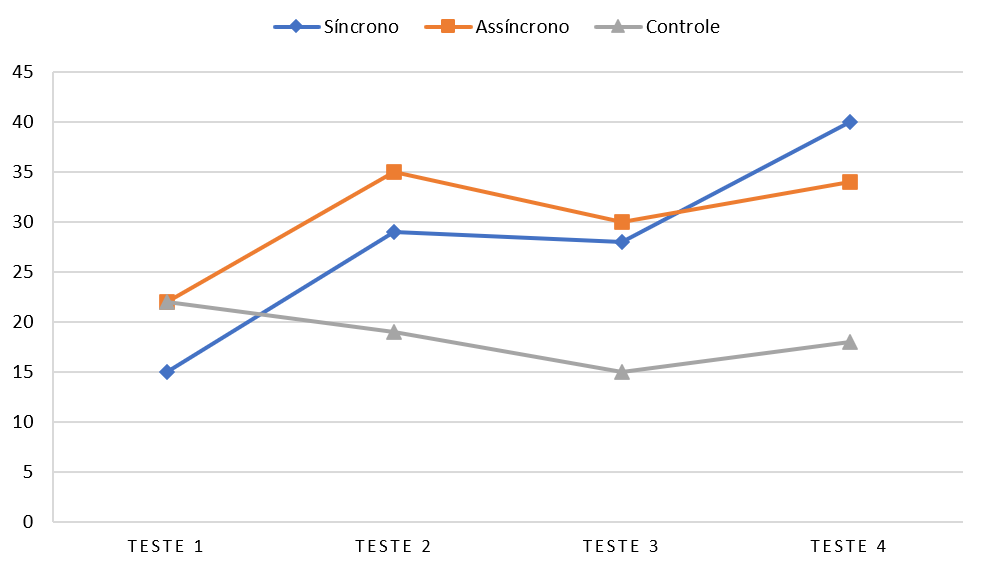
\includegraphics[width=0.75\textwidth]{fig03.png}
 \caption{Number of correct answers from Spanish groups.}
 \label{fig03}
 \source{Own elaboration.}
\end{figure}

\begin{figure}[htbp]
 \centering
 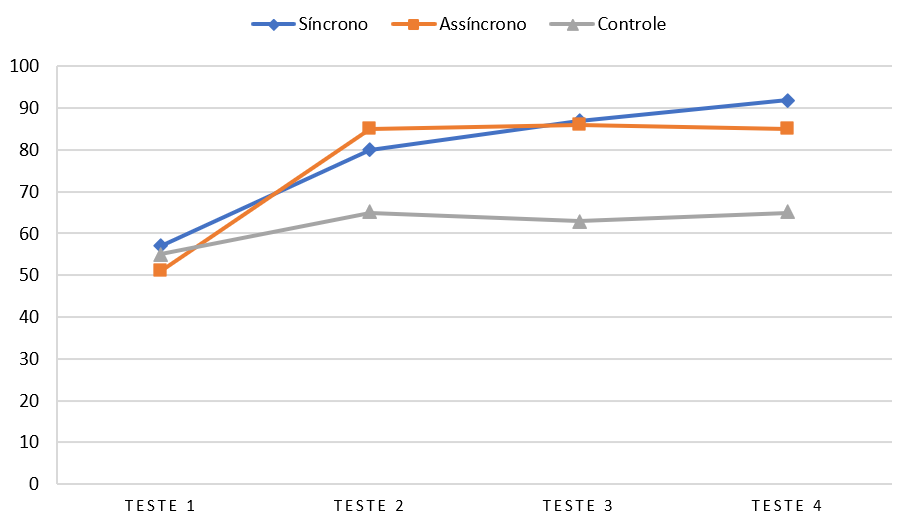
\includegraphics[width=0.75\textwidth]{fig04.png}
 \caption{Number of correct answers from English groups.}
 \label{fig04}
 \source{Own elaboration.}
\end{figure}




When analysing the learning progress in Spanish, the Friedman test
\cite{friedman_comparison_1940} showed that results differed between the 4 tests
[$X^2(3) = 10,390$; $p = 0.016$], especially in questions 1 [$X^2(3) = 10.909$; 
$p = 0.012$], 2 [$X^2(3) = 18.600$; $p < 0.001$], 3
[$X^2(3) = 16.615$; $p = 0.001$], and 5 [$X^2(3) = 12.353$; $p = 0.006$].
The multiple comparison tests showed that the biggest difference was
between tests 1 and 4. The experimental groups, unlike the control
group, showed improvement in results, especially the synchronous group.

Friedman's test also showed that the English results differ between the
4 tests [$X^2(3) = 46.947$; $p < 0.001$], especially in
questions 1 [$X^2(3) = 41.687$; $p < 0.001$], 3 [$X^2(3) = 32.690$; 
$p < 0.001$], and 7 [$X^2(3) = 21.923$; $p < 0.001$]. 
Multiple comparison tests proved that test 1 differed from
tests 2, 3 and 4. Again, the experimental groups, unlike the control
group, showed improvement in results.

\Cref{tbl07,tbl08} show the distribution of errors in the four writing
tests by number of students in each test. The most important mistakes
found were the lack of pronouns, the use of wrong or unnecessary
pronouns, the creation of ambiguity, and excessive nominal repetition.

\begin{table}[htpb]
\caption{Writing tests in Spanish.}
\label{tbl07}
\small
\centering
\begin{tabular}{lllllllllllll}
\toprule
 & \multicolumn{4}{c}{Synchronous (N=5)} & \multicolumn{4}{c}{Asynchronous (N=5)} & \multicolumn{4}{c}{Control (N=5)} \\
 & T1 & T2 & T3 & T4 & T1 & T2 & T3 & T4 & T1 & T2 & T3 & T4 \\
Lack of pronoun & 3 & 2 & 4 & 2 & 2 & 2 & 1 & 0 & 1 & 2 & 3 & 4 \\
Wrong pronoun & 3 & 4 & 2 & 2 & 2 & 3 & 0 & 3 & 1 & 4 & 3 & 3 \\
Unnecessary pronoun & 3 & 4 & 4 & 3 & 2 & 2 & 1 & 1 & 2 & 1 & 0 & 2 \\
Ambiguity & 0 & 0 & 0 & 1 & 0 & 1 & 0 & 0 & 0 & 2 & 0 & 1 \\
Nominal repetition & 5 & 4 & 4 & 5 & 5 & 3 & 2 & 5 & 5 & 5 & 5 & 5 \\
\bottomrule
\end{tabular}
\source{Own elaboration.}
\end{table}


\begin{table}[htpb]
\caption{Writing tests in English.}
\label{tbl08}
\small
\centering
\begin{tabular}{lllllllllllll}
\toprule
 & \multicolumn{4}{c}{Synchronous (N=10)} & \multicolumn{4}{c}{Asynchronous (N=10)} & \multicolumn{4}{c}{Control (N=10)} \\ 
 & T1 & T2 & T3 & T4 & T1 & T2 & T3 & T4 & T1 & T2 & T3 & T4 \\ 
Lack of pronoun & 1 & 3 & 0 & 2 & 0 & 5 & 4 & 1 & 1 & 2 & 1 & 3 \\
Wrong pronoun & 0 & 2 & 0 & 1 & 1 & 1 & 1 & 0 & 0 & 0 & 0 & 3 \\
Unnecessary pronoun & 0 & 1 & 0 & 0 & 1 & 1 & 2 & 1 & 1 & 1 & 2 & 1 \\ 
Ambiguity & 2 & 1 & 0 & 0 & 0 & 1 & 0 & 0 & 1 & 2 & 0 & 0 \\
Nominal repetition & 9 & 8 & 8 & 9 & 8 & 7 & 7 & 10 & 5 & 8 & 10 & 9 \\
\bottomrule
\end{tabular}
\source{Own elaboration.}
\end{table}


Both Spanish and English students who participated in the experimental
groups learned to identify and correct unnecessary pronouns and nominal
repetitions in the first part of the tests. However, in the second part,
which consisted of textual productions of 100 to 150 words, the set of
errors found is very small and does not seem to allow for significant
patterns in the evolution of the learning process. It should be noted,
however, that almost all students have repeated the same nouns at least
three times in their texts. Such behaviour was constant in all four
tests. This can be interpreted as demonstrating that, although the
course contributed to improving reading in a foreign language, it did
not seem to have significantly contributed to improving writing.

At the end of the \emph{Moodle} course page, students were able to
anonymously evaluate the course and the teacher. Of the 30 experimental
group participants, 19 sent their responses, of which 13 were from
English and 6 from Spanish learners. Their feedback is analysed in
\textcite{bruscato_ensino_2020} and, in general, students' perception of
the course was very positive. One student from each language, however,
would have liked the tests to have been of different text genres, so
that they could better practice what they learned. Nonetheless, it was
decided to use the same genre for all the tests so this would not become
a possible variable in the analysis of the results.

Through the teacher's subsequent analysis of the classes, it was noticed
that there was a better interaction between participants in the Spanish
synchronous group, which had 5 students, and in the English asynchronous
group, which had 10. With a smaller group, everyone can see and speak to
one another during the lesson. With a larger group, the written debates
on the forums seem to be more fruitful.

\section{Conclusion}\label{sec-conclusion}
As it was seen in the literature review, little research has been done
on the impact of learning modalities and individual student
characteristics on learning anaphoric processes in a foreign language.
However, since anaphora is one of the mechanisms responsible for textual
cohesion and is considered a sign of speakers' communicative competence,
studies focusing on this discursive mechanism are relevant for language
teaching.

This article presented the results of an experimental study on the
learning of anaphora in English and Spanish. It aimed to answer how
learning outcomes can be affected by the distance learning modality
(Q1), the foreign language studied (Q2), the assessment of reading or
writing (Q3), the level of proficiency in the foreign languages (Q4),
and the participants' degree of motivation (Q5). Thus, an online course
was offered as intervention to Modern Language students at a Brazilian
university in the first semester of 2020. The research included 1
initial questionnaire, 2 lessons of 90 minutes each, and 4 written
tests. Data from three groups were compared: one that had synchronous
lessons on the topic; one that had asynchronous lessons; and another
that had no lessons, serving only as a control group.


A positive and moderate correlation between the learners' proficiency in
the foreign language and their knowledge of anaphora was identified in
this study, as it was previously observed by \textcite{pretorius_english_2005}. In the
learner corpus compiled for the research, it was perceived that
students do not usually make errors of anaphoric ambiguity but make
excessive use of nominal repetition, confirming what was found in \textcite{lozano_2016}.

In the first part of the pretest, which contained 10 errors of different
types to assess reading, no English student noticed errors number 1 and
3, of unnecessary subject pronoun and nominal repetition, and few
Spanish students noticed them (40\% and 20\%, respectively). In the
final test, almost all students in the experimental groups got right
questions 1 (90\%) and 3 (90\% Spanish and 80\% English). Although they
noticed and corrected the excessive nominal repetition in the reading
tests, they did not do the same in their writing (second part of each
test).

Through the analysis of the tests, it has been possible to answer the
research questions (Q) raised here. A positive and moderate correlation
was identified between the students' knowledge of anaphora, level of
proficiency (Q4), and degree of motivation to study the language (Q5),
more specifically the constructs Task Value and Self-efficacy for
Learning and Performance. These correlations were noticed in the four
tests, in which students with the highest general knowledge of the
language and the highest motivation to study it showed the best results.

English students demonstrated a greater prior knowledge of anaphora than
Spanish students (Q2), probably because they have been studying it for
longer than the others; and they also presented the best results on the
tests, reaching the final score above 80\% on the reading test. Although
the experimental groups showed improvement in the reading tests, the
same did not happen with writing (Q3). A better progress in learning was
identified in the synchronous groups (Q1), which achieved the highest
scores on the final test (80\% and 92\%), but the difference with the
asynchronous groups was not significant ($p < 0.05$).

Although both distance learning modalities seem to be equally effective
for students' learning, they have different requirements. For
synchronous learning, it is necessary to connect a professor and a group
at the same time, and it is better to have smaller groups to improve
communication. For asynchronous learning, a professor must initially
prepare many study materials and activities, but a tutor can track
students' progress and answer students' questions. For institutions,
asynchronous learning seems economically the best option. However,
synchronous learning offers a contact between students and professors
that is more similar to face-to-face interaction.

This study contributes to the field by considering multiple variables to
analyse the effectiveness of distance learning modalities. However, it
has some limitations. The course only had two lessons, which did not
seem enough to improve writing in the foreign language. Furthermore,
there was a small number of participants: only 15 Spanish students and
30 English students. For the continuity of the work, it is intended to
replicate the research in Portugal to compare the results and consider
the native language variety and the educational context as other
possible variables.

\section*{Acknowledgements}
We would like to thank the professors and students of the Language
Institute at the Federal University of Rio Grande do Sul for their
collaboration in this research, in particular Dr. Sergio Menuzzi,
Director of the Faculty, for his support in the implementation and
accreditation of the course.
Jorge Baptista’s work is supported by national funds through FCT, \textit{Fundação para
a Ciência e a Tecnologia}, under project UIDB/50021/2020.

\printbibliography\label{sec-bib}
% if the text is not in Portuguese, it might be necessary to use the code below instead to print the correct ABNT abbreviations [s.n.], [s.l.] 
%\begin{portuguese}
%\printbibliography[title={Bibliography}]
%\end{portuguese}


\end{document}
